\documentclass[pre,aps,reprint,noshowpacs,superscriptaddress,floatfix,letterpaper,longbibliography]{revtex4-2}
\usepackage{amsmath,amssymb,amsbsy,amsfonts,amsthm,bbm,bm,mathtools,mathrsfs}
 % To determin margin size: 
 %\usepackage[top=1cm, bottom=1cm, left=1cm, right=1cm]{geometry} 
 \usepackage{color}
\usepackage{physics}
\usepackage{xfrac}
\usepackage[dvipsnames]{xcolor}
\definecolor{LapisLazuli}{RGB}{47, 102, 169}
\usepackage[colorlinks=true,citecolor=LapisLazuli,linkcolor=LapisLazuli,urlcolor=LapisLazuli]{hyperref} 
\usepackage{empheq}
\usepackage{pgfplots}
\usepackage{stackengine}
\usepackage{relsize}
\usepackage[inline]{enumitem}
\usepackage[normalem]{ulem} % Comment this out before submitting papers! (otherrwsie will cause problems with references. 
\usepackage{comment}
\usepackage{import}
\usepackage[english]{babel}
\usepackage{lipsum}  
\usepackage{mathtools} 
\usepackage{soul} % strikeout package; use \st{text}.
\usepackage{tikz}
\usetikzlibrary{decorations}
\usetikzlibrary{decorations.pathreplacing}

\renewcommand{\bibnumfmt}[1]{(#1)}
\usepackage{enumitem} 

% Macros -- you can add new ones sa much as you like 
\newcommand{\Comment}[1]{\textcolor{blue}{[JohnDoe: #1]}}
\newcommand{\TBC}{\magenta{[TBC]}} 

% Colors: 
\newcommand{\red}{\textcolor{red}}
\newcommand{\green}{\textcolor{green}}
\newcommand{\blue}{\textcolor{blue}}
\newcommand{\yellow}{\textcolor{yellow}} 
\newcommand{\magenta}{\textcolor{magenta}}

% Shortcuts
\newcommand{\NiceSubscript}{\tau_{\!\scriptscriptstyle\mathcal{A}}} 
\newcommand{\Qdot}{\dot{\mathcal{Q}}}
\newcommand{\Wdot}{\dot{\mathcal{W}}}
\newcommand{\Q}{\mathcal{Q}}
\newcommand{\W}{\mathcal{W}}

% Bold letters
\newcommand{\bp}{\boldsymbol{p}}
\newcommand{\bq}{\boldsymbol{q}}
\newcommand{\bx}{\boldsymbol{x}}
\newcommand{\bC}{\boldsymbol{C}}

% Math and Tables 
\newcommand{\cov}{\operatorname{cov}} % To mark covariance 
\newcommand{\Hquad}{\hspace{0.5em}} % Short spacing in equations
\newcommand{\HHquad}{\hspace{0.25em}} % Even shorter spacing 
\usepackage{pbox} % For breaking lines in table
\usepackage{tcolorbox}  % For a gray background textbox

\makeatletter
\def\maketitle{
\@author@finish
\title@column\titleblock@produce
\suppressfloats[t]}
\makeatother

%%%%%%%%%%%%%%%%%%%%%%%%%
\begin{document}
	
	\title{Paper title here}  
	
	\author{Author's name}
	\author{Jason~R.~Green}
	\email[]{jason.green@umb.edu}
	\affiliation{Department of Chemistry,\
		University of Massachusetts Boston,\
		Boston, MA 02125
	}
	\affiliation{Department of Physics,\
		University of Massachusetts Boston,\
		Boston, MA 02125
	}
	\date{\today}

%%%%%%%%%%%%%%%%%%%%%%%%% 
%%%%%%%%%%%%%%%%%%%%%%%%% 
\begin{abstract}	
	Abstract goes here.
	\lipsum[1-1]
\end{abstract}

\maketitle
%%%%%%%%%%%%%%%%%%%%%%%%%
%%%%%%%%%%%%%%%%%%%%%%%%%

\section{Introduction}
Introduction here Ref~\cite{Nicholson2020}

\lipsum[2-3]

%%%%%%%%%%%%%%%%%%%%%%%%%
\section{Results and Discussion}
Describe your results.  Here are some useful Latex tips, compare the code with the result in the compiled file. 
%%%%%%%%%%%%%%%%%%%%%%%%%
\subsection{Writing and referencing to equations:}  
\begin{enumerate} 

\item Sometimes it is useful to use, instead of, e.g., $W$; $\mathcal{W}$ or $\mathscr{W}$. Works for other letters too. 
    \item  Look at the spacing and the use of ``align'': 
\begin{align}
\Delta t \bar S/n&\geq k_B.\nonumber\\ 
&=\qquad\text{Boltzmann's constant}\quad >0\HHquad >1 . 
\label{EqSOvern}
\end{align}

\item \textbf{Remember to give relevant names to your equations! Not just Eq1, Eq2 etc., in the equation labels, because these might change.} 

\item Use (backslash) + \textbf{left} and \textbf{right} before parenthesise, to make their size adjustable: 
\begin{align}
[(\frac{\Qdot}{2})],\quad\text{versus}\quad \left[\left(\frac{\Qdot}{2}\right)\right] 
\label{EqParenthesiseSizes}
\end{align}
and here is how you reference to Eq.~\eqref{EqParenthesiseSizes}. 
This also work with floor/ceil and bra/kets: 
\begin{align}
\left\langle \frac{\W}{2}\right\rangle,\quad\left\lfloor e^{-\beta\W}\right\rfloor,\quad\text{and}\quad \left\lceil e^{-\beta\W}\right\rceil 
\label{EqParenthesiseSizes}
\end{align} 

\item To add matrices, see here: \href{https://www.overleaf.com/learn/latex/Matrices.}{Reference to read about matrices.} 

\item Sometime, you might have a long expression in brackets inside an equation, which spans over two lines. This is what you need to do in this case: Use (backslash) + (big/Big/Bigg). 
\begin{align}
    (A+B+C)^2&=\Big(A^2+B^2+C^2\nonumber\\ 
    &+2AB+2AC+2BC\Big)
\end{align} 
\href{https://garsia.math.yorku.ca/~zabrocki/latexpanel/latexpanel.pdf}{See more details here.}  

\item For Greek and special mathematical symbols,  \href{https://garsia.math.yorku.ca/~zabrocki/latexpanel/latexpanel.pdf}{See the list here.} 

\item Curled brackets, in math mode only, and underbrace: \\ 
$\left\{ \underbrace{(A+B+\sigma+\phi+\Phi)}_{max}=\text{max}(A+B+\sigma+\phi+\Phi)\right\}$. 

\item Cases: $f(\NiceSubscript) = \begin{cases}
  \NiceSubscript/2\bp+\bq  & \bp \text{ is even} \\
  3\NiceSubscript+\bp & \bp \text{ is odd}
\end{cases}$ 

\label{List:Equations}
\end{enumerate} 

%%%%%%%%%%%%%%%%%%%%%%%%%
\subsection{Writing correctly and efficiently in Latex:}
\begin{enumerate} 
\item Use the symbol $\sim$ in order to ``stick'' Eq. to the reference. For example: ``\verb|see Fig.~\ref{}|''. 

\item Use \verb|Eq.~\eqref{}|, NOT \verb|Eq.~\ref{}|. For figures and Tables, use \verb|Fig.~\ref{}| and \verb|Table.~\ref{}| without parenthesize. 

    \item Use $``$ (on the left) and $"$ (on the right) for quotes, NOT $"$ on both sides. 
    
\item \blue{This} \yellow{example} \magenta{shows} \green{how} \red{to use colors}. For comments, use \Comment{Comment here.}. You can also \textbf{bold}, \sout{strike out} and \textit{Italicize} text. \\ Note that sout require the ``ulem" package, and it must be removed before submitting a paper, or else it creates problems with the references.\\ Of course, you can also \underline{underline text}. 

\item Figure~\ref{fig:plot-label} shows how to add a normal figure and Fig~\ref{fig:TikzExample} shows how to add a figure with two panels using Tikz.  
 %%%%%%%%% Start normal figure 
 \begin{figure}[t!] %t!=top, h!=here, b!=bottom, tbh=Latex choses best
	\centering
	\hspace*{-0.75cm}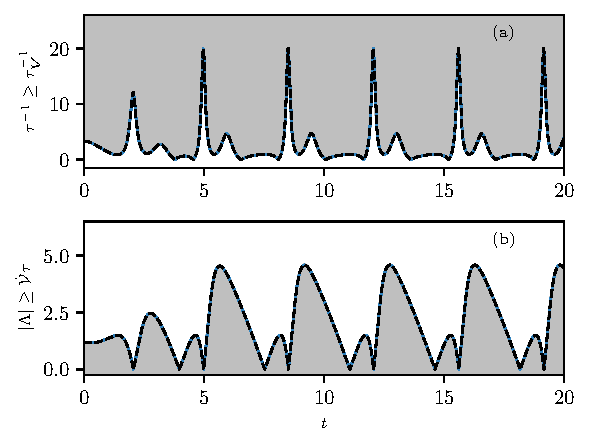
\includegraphics[width=0.45\textwidth]{sample-plot.pdf}
	\caption{\footnotesize{Caption goes here, in footnote size.}}
	\label{fig:plot-label}
\end{figure}
 %%%%%%%%% End normal figure 
 %%%%%%%%% Start Tikzfigure
\begin{figure}[tbh] %t or b or h without the "!" is a reccomendationn for top, which Latex may ignore
\centering
\begin{tikzpicture}
\node (image) at (0,-0.125) {
  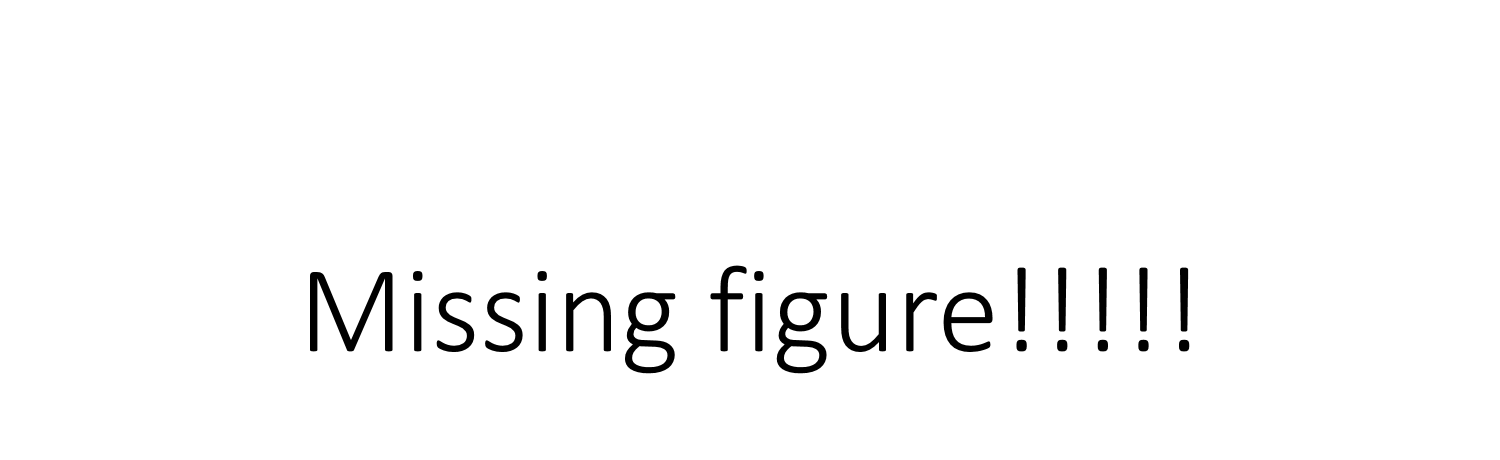
\includegraphics[width=0.9\linewidth]{MissingFigure.png}
};
\node (image) at (0,-3.75) {
  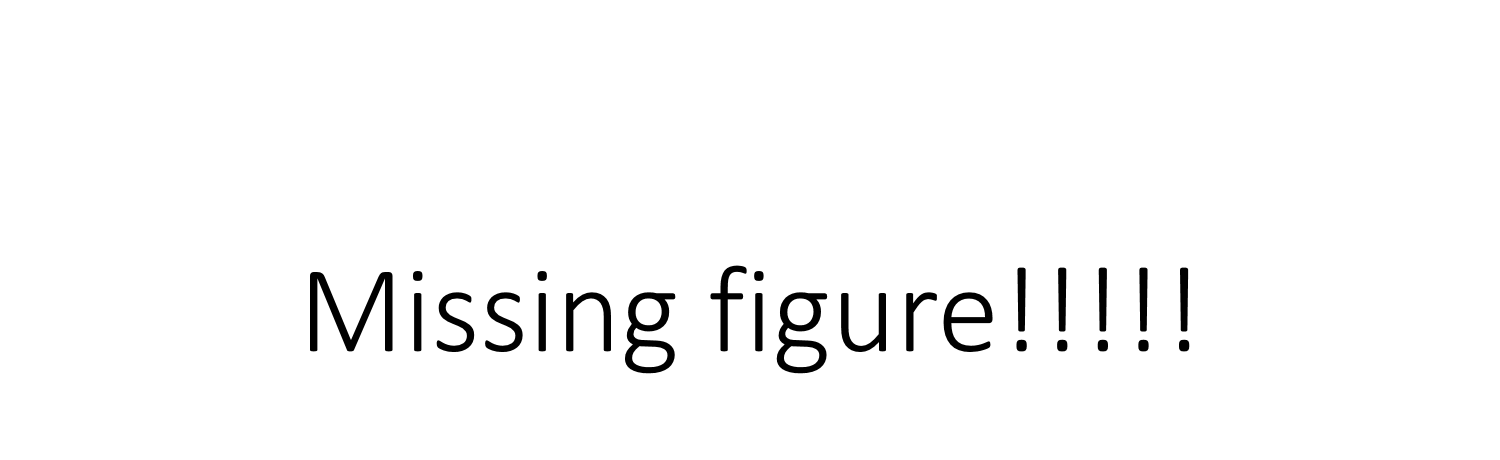
\includegraphics[width=0.9\linewidth]{MissingFigure.png}
};
\node[text=black] (a) at (-2.3,1.4){\footnotesize{(a)}};
\node[text=black] (b) at (-2.3,-2.0){\footnotesize{(b)}};
\end{tikzpicture} 
\caption{
{\footnotesize{Figure with two panels, using Tikz. Tikz helps put the '(a)' and '(b)' in the top of the panels, but can also be used to arrange the panels in general and even create pictures. ``Missing figure" is a place-holder figure (recommended to have such a figure, use your own creative designs). }}}
\label{fig:TikzExample} 
\end{figure} 
 %%%%%%%%% End Tikzfigure  

\item Say ``Figure'' at the start of a sentence and Fig. in the middle.  

\item Table~\ref{Table1} is an example for how to add tables in Latex. 
 %%%%%%%%% Start Table 
%\begin{widetext} 
%\begin{center}
\begin{table}[h!] 
\footnotesize
%\centering 
\begin{tabular}{| c | c | c |} % (3 columns) 
\hline\hline 
Category & Col$1$ & Col$2$\\
[0.5ex] %
\hline 
Cat1&$1$&$2$\\
%%%%% 
Cat2&$1$&$2$\\
%%%%% 
Cat3&$1$&$2$\\
[0.5ex]
\hline\hline 
\end{tabular} 
\caption{\footnotesize{Example of a Table.}}
\label{Table1} 
\end{table} 
%\end{center} 
%\end{widetext}
%%%%%%%%% End Table 


\item \begin{verbatim}
This is how to add codes/algorithms in Latex.
\end{verbatim} 
Use: \verb|\begin{verbatim} ..... end{verbatim}|  \\ 
or \verb|\verb|.....||. 

\st{We don't need this text.}

\item The following shows how to add bullets: 
\begin{itemize}
  \item bullet (default). 
  \item[*] Bullet (star). 
  \item[!] Bullet (exclamation mark).  
  \item[$\dagger$] Bullet (dagger). 
  \label{ListBullets}
\end{itemize}

\item To add a footnote~\footnote{All you need to do is this. (This is a footnote, not a citation.}. 

\item To add clickable links use 
\href{https://latex-tutorial.com/tutorials/hyperlinks/}{Reference to adding clickable links.} (requires the package ``hyperref"). 

\item Temporary place holder: \verb|\TBC| \\ (defined in the preamble)

\item Curled brackets, outside math mode: \verb|\{ and \} |

\item To change the margin size in a paper, use: ``usepackage[top=1cm, bottom=1cm, left=1cm, right=1cm]{geometry}"  

\item In Supplemental Material: Section titles, figures etc., are numbered as S1, S2, ... To do so, add the following lines to the preamble 
\verb|\renewcommand{\theequation}{S\arabic{equation}}|
\verb|\renewcommand{\thefigure}{S\arabic{figure}}|
\verb|\renewcommand{\thesection}{S\arabic{section}}|
\verb|\renewcommand{\thetable}{S\arabic{table}}|. 

\label{List:Latex}
\end{enumerate}

\lipsum[2-2]

%%%%%%%%%%%%%%%%%%%%%%%%%
\section{Conclusions}

Conclude the paper

\lipsum[2-3]
\\ 

%%%%%%%%%%%%%%%%%%%%%%%%%
\begin{acknowledgments}
% This text is provided by the funding agency. Jason will provide.
This material is based upon work supported by the National Science Foundation under Grant No. ....

\end{acknowledgments}

%%%%%%%%%%%%%%%%%%%%%%%%%
\bibliography{references} 

%%%%%%%%%%%%%%%%%%%%%%%%%
\appendix

%%%%%%%%%%%%%%%%%%%%%%%%%
\section{Title here}
\label{AppAT} 
We briefly explain the derivation of.... 
\begin{align}
    &1=1!\nonumber\\ 
    &(\text{Eqs in the App should be numbered A1,A2,B1 etc.}\nonumber\\ 
    &\text{There are no appendices in a PRL layout!.)}
\end{align}

%%%%%%%%%%%%%%%%%%%%%%%%%


\clearpage
\setcounter{figure}{0}
\setcounter{section}{0}
\renewcommand{\thefigure}{SM\arabic{figure}}
\title{Supplemental Material: Paper title }
\maketitle

%\section{First section}{\label{sec:}}

\end{document}
